\documentclass[11pt]{article}
\usepackage[T1]{fontenc}
\usepackage{lmodern}
\usepackage{amsmath,amssymb,amsthm,mathtools}
\usepackage{graphicx}
\usepackage[margin=1in]{geometry}
\usepackage[colorlinks=true,linkcolor=blue,citecolor=blue,urlcolor=blue]{hyperref}
\usepackage{microtype}

\newtheorem{theorem}{Theorem}
\newtheorem{remark}[theorem]{Remark}
\newcommand{\B}{\mathcal B}
\newcommand{\C}{\mathbb C}
\newcommand{\N}{\mathbb N}
\newcommand{\Hh}{\ell_2(\N)}

\title{A diagonal counterexample to Besov spectral mapping\\
\large A negative answer to the final question in arXiv:1910.06369, Section 8.2}
\author{Automated mathematics discovery run \texttt{fa\_banach\_001}\\
Lane 5, candidate for human review}
\date{21 July 2026}

\begin{document}
\maketitle

\begin{center}
\fbox{\parbox{0.92\textwidth}{\textbf{Status: candidate counterexample, likely valid.}
For every $t>0$ the bounded diagonal operator $f(tA)$ has an extra spectral
limit point which is absent from $f(t\sigma(A))\cup\{0\}$.}}
\end{center}

\section{Source question}

Batty, Gomilko, and Tomilov define an analytic Besov algebra $\B$ and its
functional calculus for generators of bounded semigroups \cite{BGT}.  Their
Theorem 7.3 proves, under the additional hypothesis that $f$ vanishes at
infinity,
\[
 \sigma(f(A))\cup\{0\}=f(\sigma(A))\cup\{0\}.
\]
The exact formula in the source is reproduced here.

\begin{center}
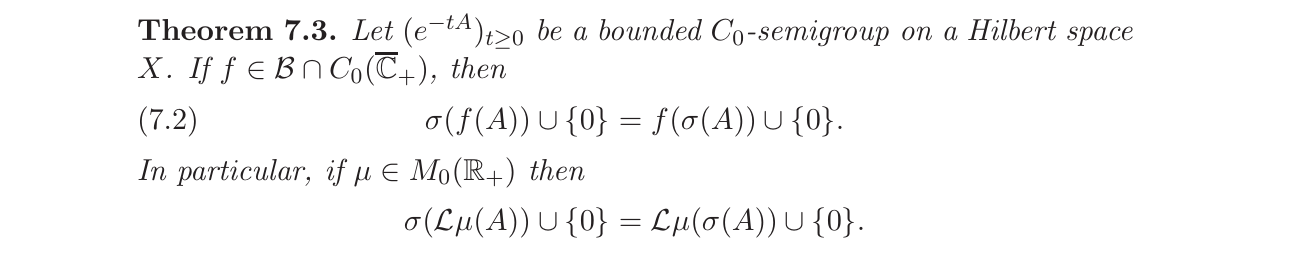
\includegraphics[width=0.94\textwidth]{figures/spectral_mapping_formula_crop.png}
\end{center}

On page 43 they ask whether the equality remains true for $f(tA)$ if
$f\in\B$ and $t\mapsto f(tA)$ is norm-continuous on $(0,\infty)$.

\begin{center}

\includegraphics[width=0.96\textwidth]{figures/open_problem_crop.png}
\end{center}

We answer this final explicitly stated question negatively, in the simplest
normal diagonal setting.

\section{Statement and proof intuition}

Recall the source definition
\[
 \B=\left\{f\in\operatorname{Hol}(\C_+):
 \int_0^\infty\sup_{\beta\in\mathbb R}
 |f'(\alpha+i\beta)|\,d\alpha<\infty\right\},
\]
with norm given by the displayed seminorm plus $\|f\|_\infty$.

\begin{theorem}\label{thm:main}
There exist a bounded $C_0$-semigroup with negative generator $-A$ on a
Hilbert space and $f\in\B$ such that
\[
 t\longmapsto f(tA)\quad\text{belongs to }C((0,\infty),\mathcal L(X)),
\]
but, for every $t>0$,
\[
 \sigma(f(tA))\cup\{0\}\ne f(t\sigma(A))\cup\{0\}.
\]
\end{theorem}

\paragraph{Proof intuition.}
Choose an unbounded discrete spectrum and a Besov function with a nonzero
limit at infinity.  The values of $f$ on the discrete spectrum converge to
that limit.  Hence the spectrum of the resulting bounded diagonal operator,
which is the closure of its diagonal entries, acquires one extra point.
The exact rational formula makes the dilation family norm-continuous away
from zero.  Thus norm continuity does not repair the missing ``point at
infinity'' in the proposed spectral image.

\section{Proof}

Let $X=\Hh$, with canonical basis $(e_n)_{n\ge1}$, and define
\[
 Ae_n=in e_n,\qquad
 D(A)=\left\{x=(x_n):\sum_{n\ge1}n^2|x_n|^2<\infty\right\}.
\]
Then $A$ is closed and densely defined, and
\[
 T(s)e_n=e^{-ins}e_n\qquad(s\ge0)
\]
is a unitary $C_0$-semigroup with generator $-A$.  Strong continuity follows
immediately from dominated convergence applied to
$\sum_n|e^{-ins}-1|^2|x_n|^2$.

Take
\[
 f(z)=\frac{z}{1+z}=1-\frac1{1+z}.
\]
For $z=\alpha+i\beta$ in $\C_+$,
\[
 f'(z)=\frac1{(1+z)^2},\qquad
 \sup_{\beta\in\mathbb R}|f'(\alpha+i\beta)|=(1+\alpha)^{-2}.
\]
Consequently
\[
 \int_0^\infty\sup_\beta|f'(\alpha+i\beta)|\,d\alpha=1.
\]
Moreover $|z|<|1+z|$ on $\C_+$, so $\|f\|_\infty=1$.  Thus $f\in\B$,
and its value at infinity is $f(\infty)=1$.

Compatibility of the $\B$-calculus with the resolvent calculus
\cite[Theorem 1.1(b)]{BGT} gives, for $t>0$,
\[
 f(tA)=I-(I+tA)^{-1},\qquad
 f(tA)e_n=b_n(t)e_n,
 \quad b_n(t):=\frac{itn}{1+itn}.
\]
If $s,t>0$, then
\begin{align*}
 |b_n(t)-b_n(s)|
 &=\frac{|t-s|n}{\sqrt{1+t^2n^2}\sqrt{1+s^2n^2}}\\
 &\le \frac{|t-s|}{\min\{s,t\}}.
\end{align*}
The operator norm of a bounded diagonal operator is the supremum of the
moduli of its entries.  Taking the supremum over $n$ therefore proves that
$t\mapsto f(tA)$ is norm-continuous on $(0,\infty)$.

The spectrum of the unbounded diagonal operator is
\[
 \sigma(A)=\{in:n\ge1\}.
\]
Indeed, away from this closed discrete set the diagonal inverse of
$A-\lambda$ is bounded.  A bounded diagonal operator has spectrum equal to
the closure of its diagonal entries: outside that closure the coordinatewise
inverse is bounded, while points in the closure are eigenvalues or approximate
eigenvalues.  Since $b_n(t)\to1$,
\[
 \sigma(f(tA))=\{b_n(t):n\ge1\}\cup\{1\}.
\]
In particular $e_n$ is an approximate eigenvector sequence at $1$, because
\[
 \|(f(tA)-I)e_n\|=|b_n(t)-1|=\frac1{\sqrt{1+t^2n^2}}\longrightarrow0.
\]
On the other hand,
\[
 f(t\sigma(A))\cup\{0\}=\{b_n(t):n\ge1\}\cup\{0\}.
\]
The point $1$ does not occur on the right: $b_n(t)=1$ would imply
$itn=1+itn$.  Thus the two sets differ for every $t>0$, proving
Theorem~\ref{thm:main}. \qed

\section{Scope, verification, and novelty}

The mechanism is exactly excluded by the positive Theorem 7.3 in the source:
that theorem assumes $f\in\B\cap C_0(\overline{\C}_+)$, whereas here
$f(\infty)=1$.  Adding $\{0\}$ cannot conceal the nonzero extra point.

There is one interpretive caveat.  The paragraph containing the question
first refers to Theorem 8.8, where a resolvent-decay hypothesis is a sufficient
condition for norm continuity, and then asks the final question using only
$f\in\B$ and norm continuity.  The example answers that final formulation.
It does not satisfy the stronger decay condition: for fixed $\alpha>0$ and
$\beta=n$, the relevant diagonal resolvent has norm $1/\alpha$, while
$|f(\alpha+in)|\to1$.  No claim is made about a strengthened reading that
retains that extra condition.

The included deterministic checker verifies the scalar identities,
continuity bound, and convergence to the extra point.  The proof itself is
exact and does not depend on computation.

The run indexes were searched by arXiv id, title, and core terms.  A bounded
primary arXiv search used the exact question, source title, authors, and
related Besov-calculus papers; it found no explicit answer or this diagonal
example.  This is not an exhaustive novelty certification.  We recommend
human review, with priority given to the intended scope of the opening
Theorem 8.8 reference.

\begin{thebibliography}{9}
\bibitem{BGT}
C. Batty, A. Gomilko, and Yu. Tomilov,
\emph{The theory of Besov functional calculus: developments and applications
to semigroups}, arXiv:1910.06369 (2019; revised 2021).
\end{thebibliography}

\end{document}
